\section{Lecture 1: Basic Concepts About Matter}

\subsection{Matter}

\begin{defn}
\textit{Matter} is anything that has mass and occupies space. The \textit{mass} of an object is the measure of the amount of matter in an object, and the \textit{volume} of an object is the amount of space the object takes up in three-dimensional space.
\end{defn}

\noindent
\note{Matter includes living, nonliving, viewable, and non-viewable things, such as wood, rocks, gasoline, air, bacteria, etc.}

\subsection{The Three States of Matter}

\begin{itemize}
\item \textbf{Solids} have \textit{definite shape and definite volume}, and have \textit{the least energy} out of the three states.
\item \textbf{Liquids} have \textit{indefinite shape but definite volume} by taking the shape of its container, and thus, they have \textit{more energy than solids but less energy than gases.}
\item \textbf{Gases} have \textit{indefinite shape and indefinite volume} as they expand to take the shape and volume of their container, and thus, they have \textit{the most energy} of the three types.
\end{itemize}

\noindent
\note{As the temperature of matter increases, particles move faster as they have more energy. Particles in solids have a lower/near-zero velocity, but particles in gases or liquids will have higher velocities and thus higher energies.}

\subsection{The Properties of Matter}

The properties of matter are the distinguishing characteristics of a substance, and they are useful for the identification/classification of unknown substances, characterization of a newly-discovered substance, distinguishing between different substances, and predicting the usefulness of a substance for a specific purpose. \\

\noindent
\note{Properties of Matter are split into two types: \textbf{Physical} and \textbf{Chemical}.}

\begin{defn}
A \textbf{physical property} is a characteristic of a substance that can be observed without changing the substance into another substance \textit{chemically}. A \textbf{chemical property}  describes the way a substance undergoes a change into another substance.
\end{defn}

\begin{figure}[H]
	\centering
	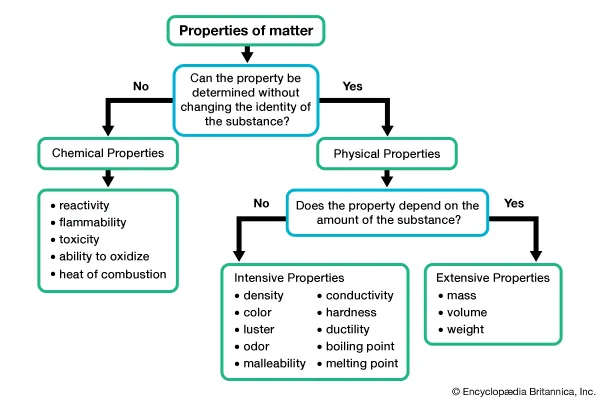
\includegraphics[width=0.9\textwidth]{matter_flowchart}
	\caption{Properties of Matter Flowchart. \note{Remember the difference between Intensive and Extensive physical properties}}
\end{figure}

\subsection{Changes in Matter}

Physical changes to matter change a substance's physical appearance but not its chemical composition, and chemical changes affect its chemical composition (and usually additionally change its physical qualities in the process) \textbf{to form a completely new substance}. Physical changes include melting ice, forming clouds, cutting, breaking, etc. Chemical changes include heating/cooking, reacting a substance with another substance, healing a wound, rusting, fermentation, etc. \\

\noindent
\note{Remember that the key difference between physical and chemical changes is whether or not a new substance is formed by the change.} \\

\noindent
\note{Dissolving salt into water is actually a chemical change because when salt dissolves, it dissociates into ions, thus changing its chemical composition, but dissolving sugar into water is physical because the sugar simply changes from a solid state to an aqueous state.}

\subsubsection{Naming Changes Between Matter States}

The movement from each state of matter to another has a completely different term based on the nature of the change.

\begin{figure}[H]
	\centering
	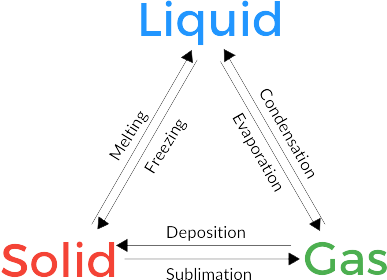
\includegraphics[width=0.6\textwidth]{state_triangle}
	\caption{States of Matter Flowchart}
\end{figure}

\newpage

\subsection{Pure Substances and Mixtures}

Matter can be classified into one of two types: mixtures or pure substances. Pure substances are composed of a singular substance and cannot be physically separated (think like Pure Gold). Whereas mixtures are comprised of more than one substance and can be physically separated into its component substances.

\begin{figure}[H]
	\centering
	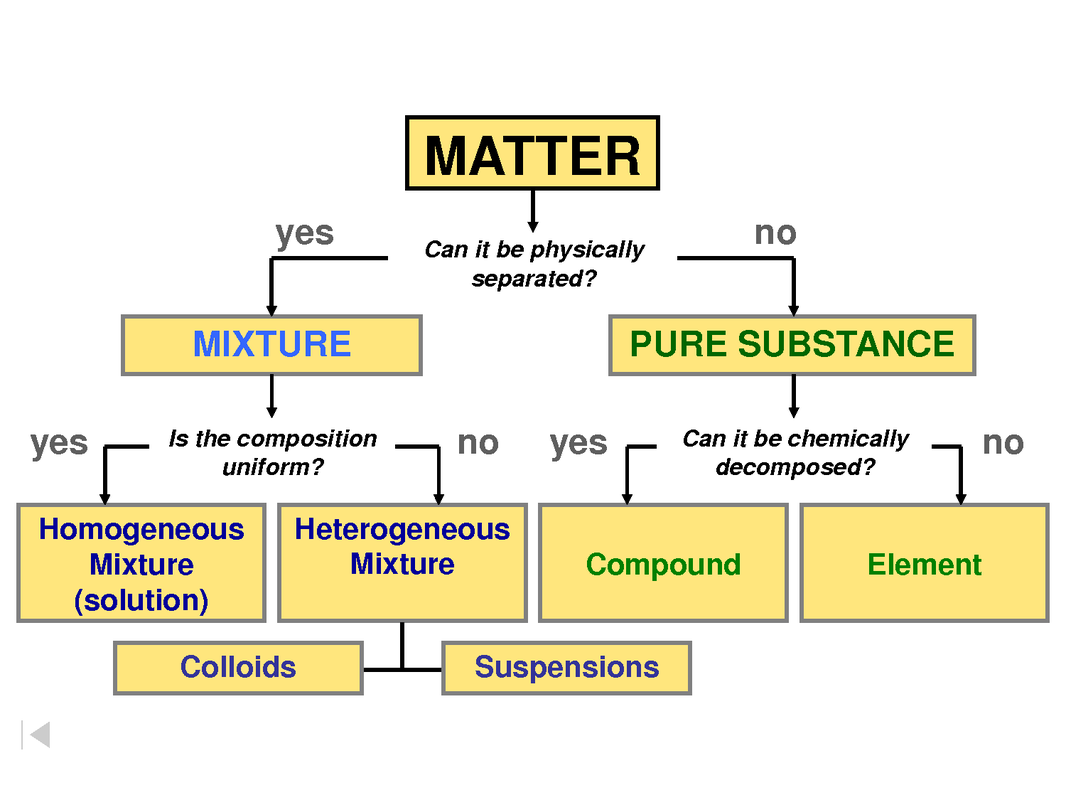
\includegraphics[width=\textwidth]{matter_types_flowchart}
	\caption{Pure Substance vs. Mixtures Flowchart}
\end{figure}

\begin{itemize}
\item \textit{Pure Substances} only ever have one substance present, and thus, have a definite and constant composition and consistent chemical and physical properties. \note{Pure substances are always chemically homogeneous, but they can be physically homogeneous or heterogeneous.}
\item \textit{Mixtures} are combinations of more than one type of substance, and thus, have variable composition and properties. \note{Mixtures are always chemically heterogeneous but, like pure substances, can be physically homogeneous or heterogeneous.}
\item \textit{Elements} are molecules with a singular \textit{type} of atom.
\item \textit{Compounds} are molecules with two or more types of atoms joined together.
\item \textit{Homogeneous Mixtures} are mixtures where a substance (known as the solute, such as salt or sugar) is dissolved into another substance (known as the solvent, such as water) at a \textit{uniform distribution} (think saltwater). These mixtures are also known as \textbf{solutions} and have one distinct physical appearance (or phase).
\item \textit{Heterogeneous Mixtures} are non-solution mixtures with a non-uniform distribution of its comprising particles and thus, two or more distinct physical appearances/phases (think Chex Mix).
\end{itemize}

\subsection{Elements and Compounds}

\begin{defn}
Elements are the building blocks of all higher types of matter and are made from atoms. They are the smallest classification of substances, and thus, cannot be broken down into simpler substances through chemical or physical means. \note{There are currently 118 known atom types, and 90 of those types occur naturally in nature.}
\end{defn}

